%!TEX root = ../dissertation.tex
\chapter{Work Plan}
\label{chapter:work_plan}

% Fazer introdução e explicar brevemente o que é o RISC-V, o CVA6
Recent advances in modern computing architectures have been powered by a new and innovative Instruction Set Architecture (ISA) called RISC-V. RISC-V stands out from other mainstream ISAs due to its accessible, free, and open standards. Its highly modularity and customizable extension scheme allow it to be used for something as simple as a low-energy consumption microcontroller to a fully capable supercomputer.

An open-source project based on the RISC-V ISA is the "CVA6 project". Its objective is to develop a set of production quality, open source, application class RISC-V CPU cores. The CVA6 is a processor architecture that is described in SystemVerilog language and it can be heavily customized. The base version of this processor has the ability to be either 32-bit or 64-bit with or without floating point support.

The CVA6 is a 6-stage, single-issue CPU that implements the RISC-V instruction set and can be configured to run in either 32-bit or 64-bit with support for floating point operations. It fully implements I, M, and C extensions of RISC-V as well as a three-level privilege system.

The CPU has a scoreboard that helps to hide the access latency to the data RAM. It does so by issuing data-independent instructions. The instruction RAM has a low access latency of 1 cycle on a hit. However, accessing the data RAM (or L1 data cache) has a longer latency of 3 cycles on a hit.


\begin{figure}[H]
	\begin{center}
 		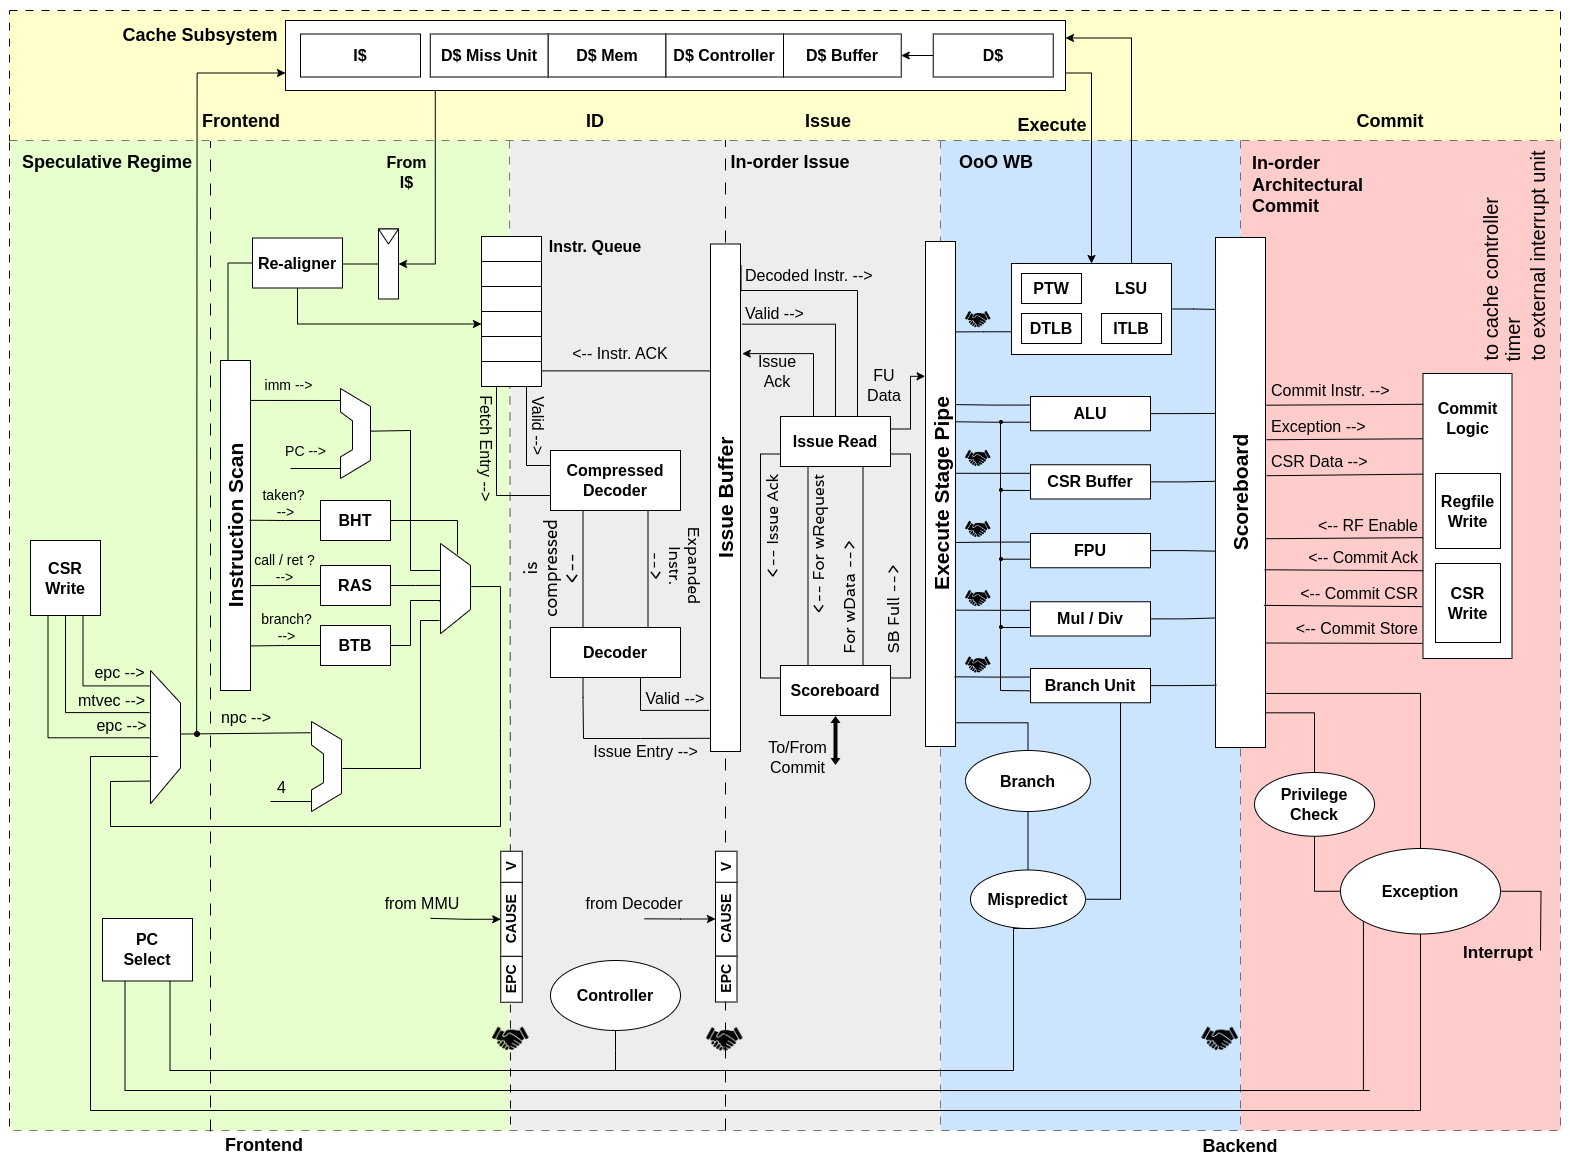
\includegraphics[width=0.7\linewidth]{images/cva6_overview.png}
 		\caption{Overview of the 6-stage pipeline of CVA6}
 		\label{fig:cva6-overview}
	\end{center} 
\end{figure}


\section{RISC-V with UVE Support}
\section{Proposed Architecture}
\section{CVA6 Implementation of Purposed Streaming Engine }
%\section{Preliminary Tests on CVA6}

-Matrix vector Multiply
-sparse matrix
-matrix multiply